%%%%%%%%%%%%%%%%%%%%%%%%%%%%%%%%%%%%%%%%%%%%%%%%%%%%%%%%%%%%%%%%%%%%%%%%%%%%%%%%%%
\begin{frame}[fragile]\frametitle{}
\begin{center}
{\Large Parsing is the key}

{\tiny (Ref: Key to RAG Success: Document Parsing Explained - EyeLevel )}
\end{center}
\end{frame}

%%%%%%%%%%%%%%%%%%%%%%%%%%%%%%%%%%%%%%%%%%%%%%%%%%%%%%%%%%%
\begin{frame}[fragile]\frametitle{Document Parsing: The Foundation of RAG}

\begin{columns}
    \begin{column}[T]{0.5\linewidth}
	  \begin{itemize}
		\item Parsing is the first step in any RAG pipeline.
		\item Bad parsing undermines even the best RAG strategies.
		\item Garbage in, garbage out: poor inputs = poor outputs.
		\item Many overlook parsing in favor of flashy AI tools.
		\item Without good extraction, nothing else matters.
	  \end{itemize}

    \end{column}
    \begin{column}[T]{0.5\linewidth}
	  \begin{itemize}
		\item Most language models require clean, structured text.
		\item RAG applications depend on text quality from source docs.
		\item Advanced RAG still fails without reliable input.
		\item Models can't fix broken, messy data.
		\item Real-world systems have failed due to poor parsing.
	  \end{itemize}
    \end{column}
  \end{columns}
  

\end{frame}

%%%%%%%%%%%%%%%%%%%%%%%%%%%%%%%%%%%%%%%%%%%%%%%%%%%%%%%%%%%
\begin{frame}[fragile]\frametitle{What is Document Parsing?}

	  \begin{itemize}
		\item Converts formats like PDF, DOCX, HTML into usable text.
		\item Extracts meaningful content for language model input.
		\item Cleans, structures, and normalizes the data.
		\item Essential step before chunking or embedding.
		\item Involves handling many formats and edge cases.
	  \end{itemize}


		\begin{center}
		  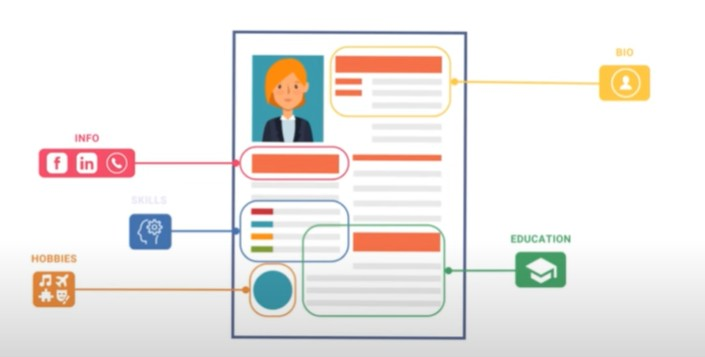
\includegraphics[width=0.8\linewidth,keepaspectratio]{rag_parsing1}
		  
		{\tiny (Ref: Key to RAG Success: Document Parsing Explained - EyeLevel )}
		  
		\end{center}
  
\end{frame}

%%%%%%%%%%%%%%%%%%%%%%%%%%%%%%%%%%%%%%%%%%%%%%%%%%%%%%%%%%%
\begin{frame}[fragile]\frametitle{Common Misconceptions}
  \begin{itemize}
    \item Engineers often ignore parsing during development.
    \item Focus tends to be on model tuning or retrieval logic.
    \item Parsing is wrongly assumed to be solved or trivial.
    \item Most systems lack formal evaluation of parsers.
    \item Homemade or ad-hoc solutions dominate practice.
  \end{itemize}
\end{frame}

%%%%%%%%%%%%%%%%%%%%%%%%%%%%%%%%%%%%%%%%%%%%%%%%%%%%%%%%%%%
\begin{frame}[fragile]\frametitle{The Reddit Survey Insight}

	  \begin{itemize}
		\item Survey on LangChain subreddit revealed no consensus.
		\item 57 replies yielded 30+ different parsing techniques.
		\item Most users hacked together informal solutions.
		\item Few performed proper parser evaluation or comparison.
		\item Highlights need for standardized testing and benchmarking.
	  \end{itemize}


		\begin{center}
		  
\includegraphics[width=0.8\linewidth,keepaspectratio]{rag_parsing2}
		  
		{\tiny (Ref: Key to RAG Success: Document Parsing Explained - EyeLevel )}
		  
		\end{center}

\end{frame}

%%%%%%%%%%%%%%%%%%%%%%%%%%%%%%%%%%%%%%%%%%%%%%%%%%%%%%%%%%%
\begin{frame}[fragile]\frametitle{Popular Parsing Tools Compared}

\begin{columns}
    \begin{column}[T]{0.5\linewidth}
	  \begin{itemize}
		\item PyPDF – well-known, older, basic PDF extraction.
		\item Tesseract – OCR-based, handles scanned documents.
		\item Unstructured – handles messy formats, layout-aware.
		\item Tools vary widely in output quality and reliability.
		\item Choice depends on document type and project needs.
	  \end{itemize}

    \end{column}
    \begin{column}[T]{0.5\linewidth}
	  \begin{itemize}
		\item Start by identifying your document types.
		\item Evaluate parsers with real-world examples.
		\item Compare outputs side by side.
		\item Look for structural fidelity, cleanliness, completeness.
		\item Test rigorously — don’t rely on "it seems to work".
	  \end{itemize}
    \end{column}
  \end{columns}  
 

\end{frame}


%%%%%%%%%%%%%%%%%%%%%%%%%%%%%%%%%%%%%%%%%%%%%%%%%%%%%%%%%%%
\begin{frame}[fragile]\frametitle{Real-World Example: Medical Bill}
\begin{columns}
  \begin{column}[T]{0.6\linewidth}
    \begin{itemize}
      \item Parsing tested on de-identified medical bill.
      \item Chosen for layout complexity and format irregularities.
      \item Shows strengths and weaknesses of each parser.
      \item Realistic example of what RAG apps encounter.
      \item Highlights need for resilient parsing strategies.
    \end{itemize}
  \end{column}
  \begin{column}[T]{0.4\linewidth}
    \begin{center}
      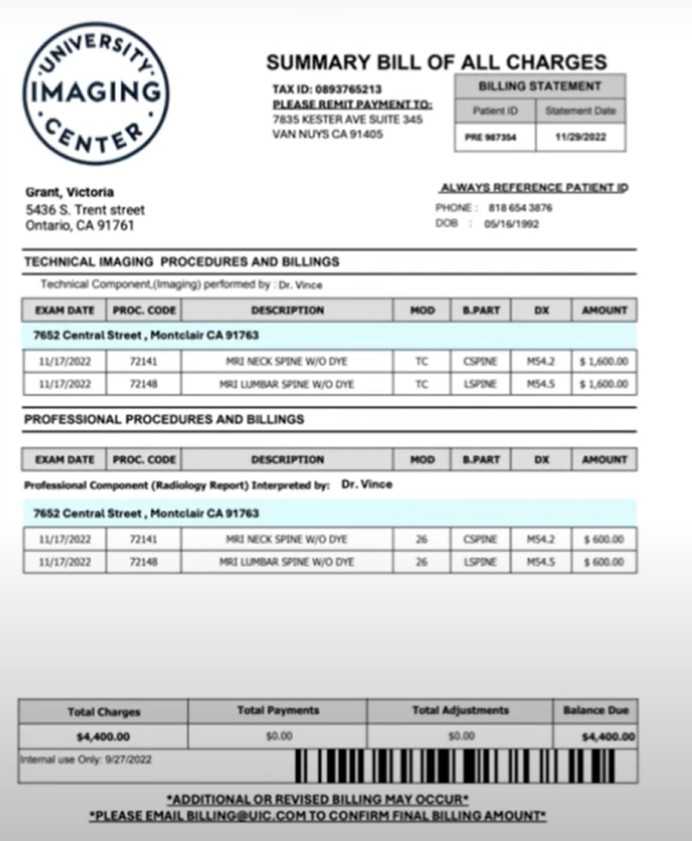
\includegraphics[width=0.8\linewidth,keepaspectratio]{rag_parsing3}
    \end{center}
  \end{column}
\end{columns}
\end{frame}

%%%%%%%%%%%%%%%%%%%%%%%%%%%%%%%%%%%%%%%%%%%%%%%%%%%%%%%%%%%
\begin{frame}[fragile]\frametitle{Limitations of PyPDF}


  \begin{itemize}
    \item PyPDF ok for texts but struggles with complex formats like tables.
    \item It failed to extract key data from real-world docs.
    \item Parsing tables often results in empty or broken content.
    \item Not due to PyPDF's fault—PDFs are inherently hard to parse.
    \item Many PDFs use inconsistent encoding and layouts.
  \end{itemize}

    \begin{center}
      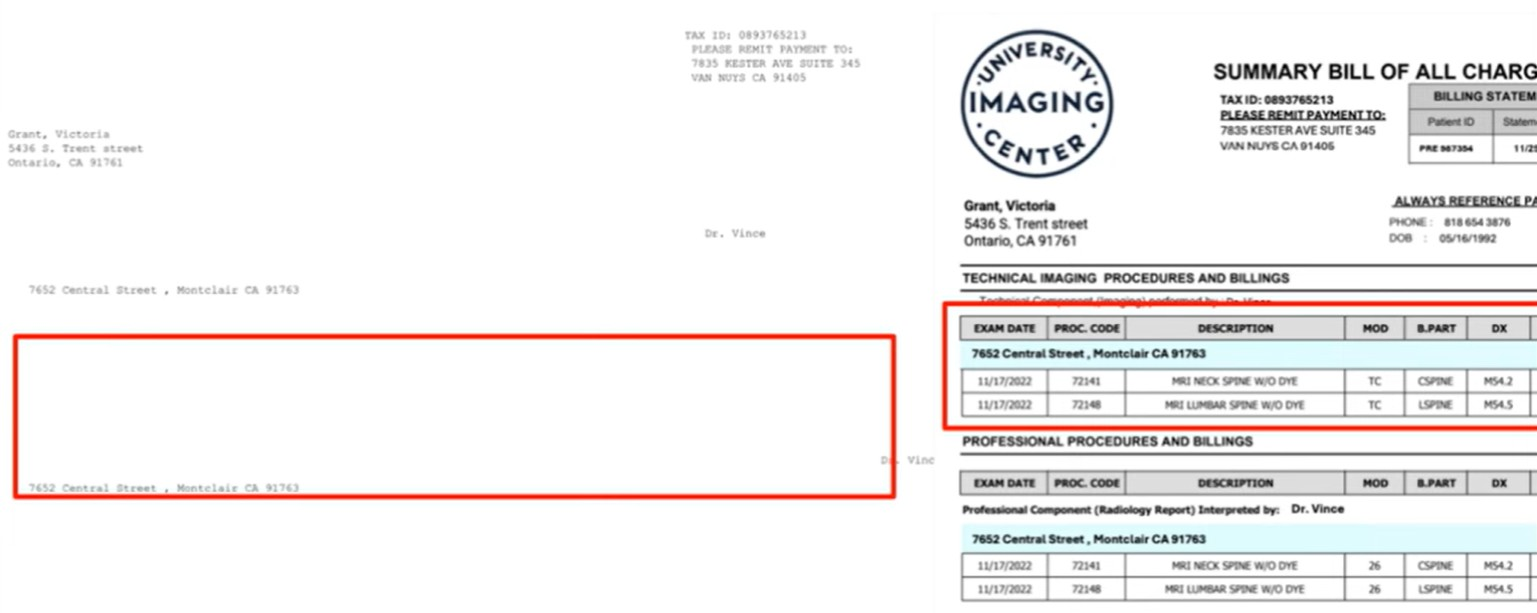
\includegraphics[width=0.8\linewidth,keepaspectratio]{rag_parsing4}
    \end{center}

\end{frame}

%%%%%%%%%%%%%%%%%%%%%%%%%%%%%%%%%%%%%%%%%%%%%%%%%%%%%%%%%%%
\begin{frame}[fragile]\frametitle{Tesseract OCR: Strengths and Weaknesses}

  \begin{itemize}
    \item Tesseract uses image-based OCR to extract text.
    \item Better at recognizing tables than PyPDF.
    \item Still introduces errors in column alignment.
    \item Column headers often get merged or misread.
    \item OCR also introduces spelling mistakes (e.g. "Cove" vs. "Code").
  \end{itemize}

    \begin{center}
      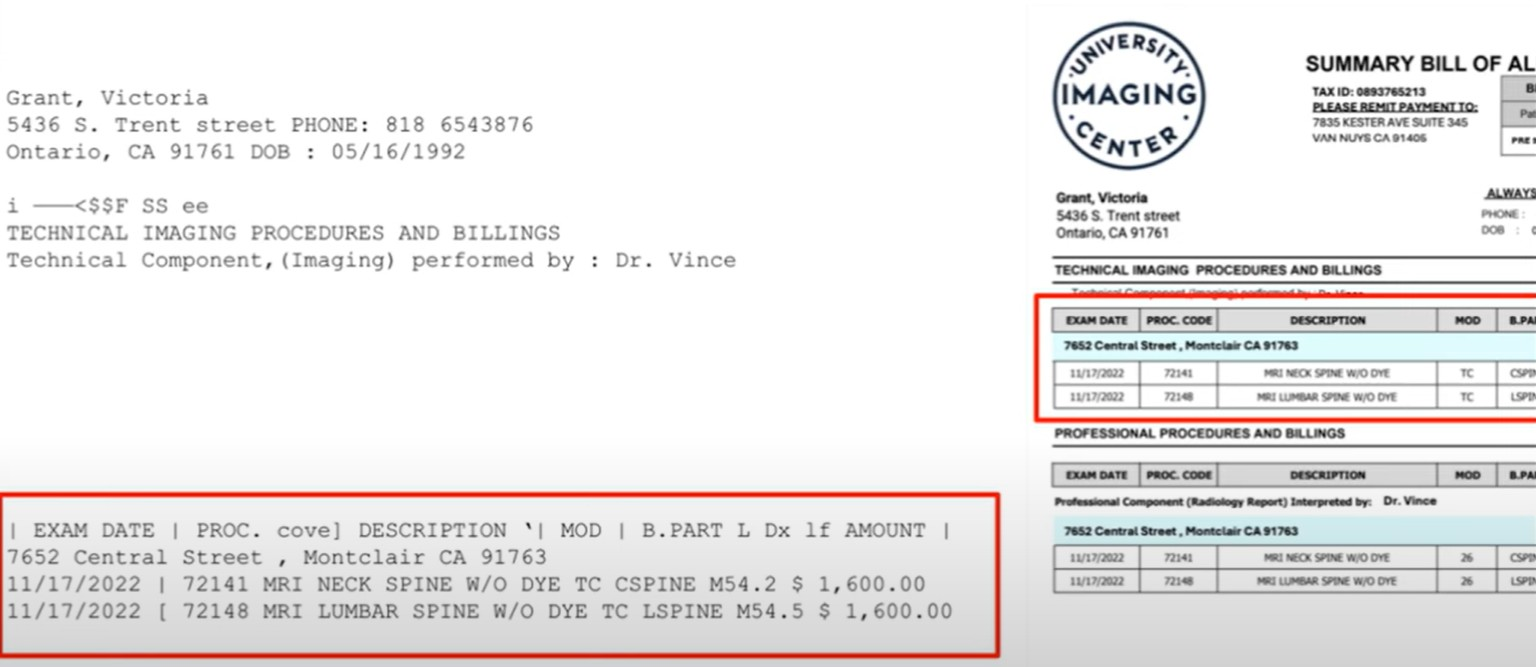
\includegraphics[width=0.8\linewidth,keepaspectratio]{rag_parsing5}
    \end{center}
 
\end{frame}

%%%%%%%%%%%%%%%%%%%%%%%%%%%%%%%%%%%%%%%%%%%%%%%%%%%%%%%%%%%
\begin{frame}[fragile]\frametitle{Challenges with OCR Outputs}
  \begin{itemize}
    \item Language models must infer structure from broken text.
    \item Humans can "guess" meaning—models may not.
    \item Noisy extractions increase risk of incorrect answers.
    \item Inconsistent column separation confuses models.
    \item Clean layout is crucial for reliable RAG responses.
  \end{itemize}
\end{frame}

%%%%%%%%%%%%%%%%%%%%%%%%%%%%%%%%%%%%%%%%%%%%%%%%%%%%%%%%%%%
\begin{frame}[fragile]\frametitle{Unstructured: A Common Default}

  \begin{itemize}
    \item Popular choice 'Unstructured' company; default in LangChain integrations.
    \item Handles layout better than OCR in some cases.
    \item Still suffers from column misalignments.
    \item Model must rely on context instead of structure.
    \item Reasonable quality, but far from perfect.
  \end{itemize}

    \begin{center}
      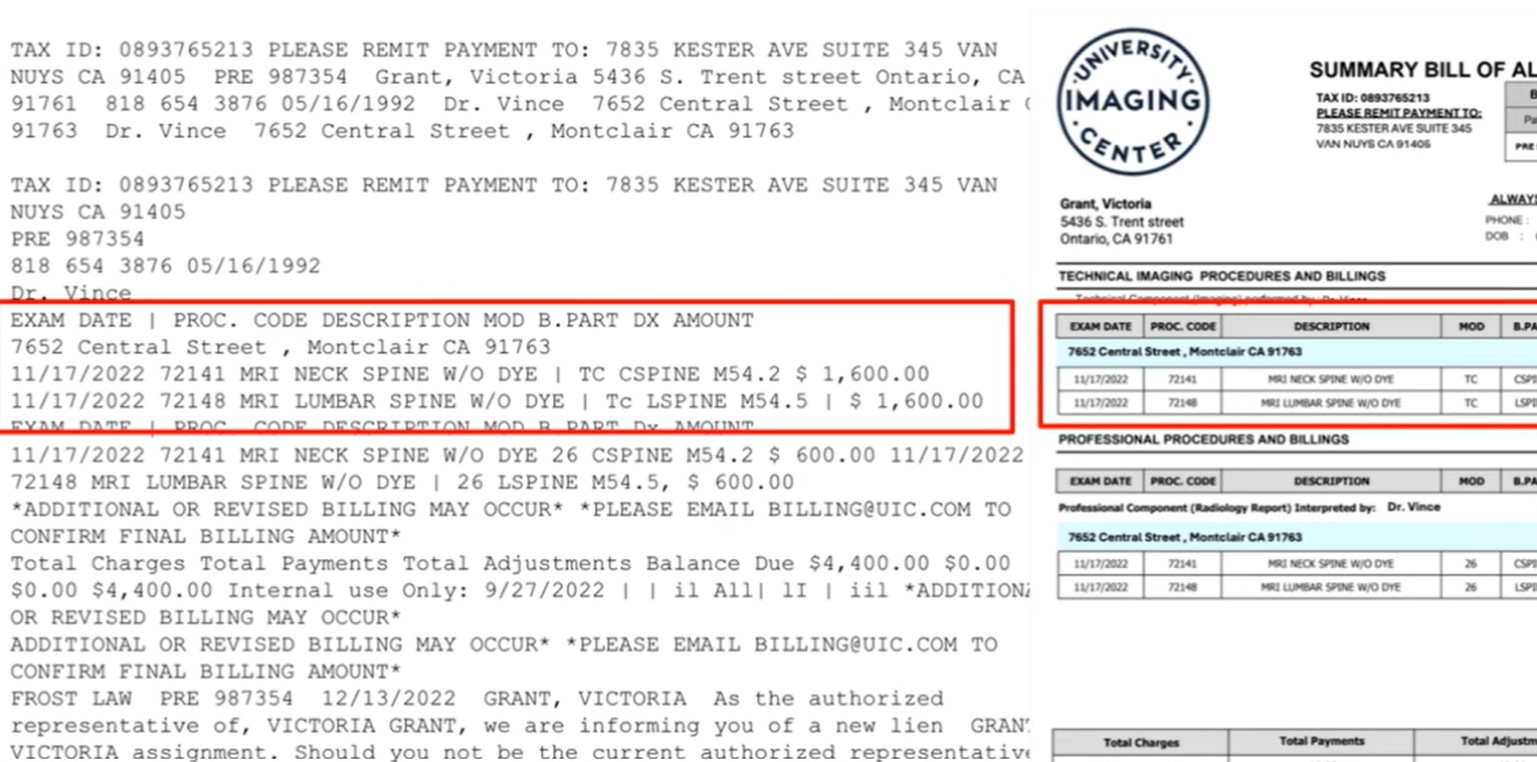
\includegraphics[width=0.8\linewidth,keepaspectratio]{rag_parsing6}
    \end{center}

\end{frame}

%%%%%%%%%%%%%%%%%%%%%%%%%%%%%%%%%%%%%%%%%%%%%%%%%%%%%%%%%%%
\begin{frame}[fragile]\frametitle{Parsing Tradeoffs: Model vs. Parser}
  \begin{itemize}
    \item Many teams focus on improving the model first.
    \item Upgrading the parser might yield better gains.
    \item Better input can reduce model burden.
    \item Smaller or older models benefit more from clean text.
    \item Strong parsing reduces reliance on inference tricks.
  \end{itemize}
\end{frame}

%%%%%%%%%%%%%%%%%%%%%%%%%%%%%%%%%%%%%%%%%%%%%%%%%%%%%%%%%%%
\begin{frame}[fragile]\frametitle{LlamaParse: Cleaner Table Extraction}

  \begin{itemize}
    \item Developed by LlamaIndex, supports markdown output.
    \item Clearly separates rows and columns with pipes.
    \item Markdown format improves model interpretability.
    \item Some formatting quirks but largely usable.
    \item Outperforms other parsers in structural clarity.
  \end{itemize}

    \begin{center}
      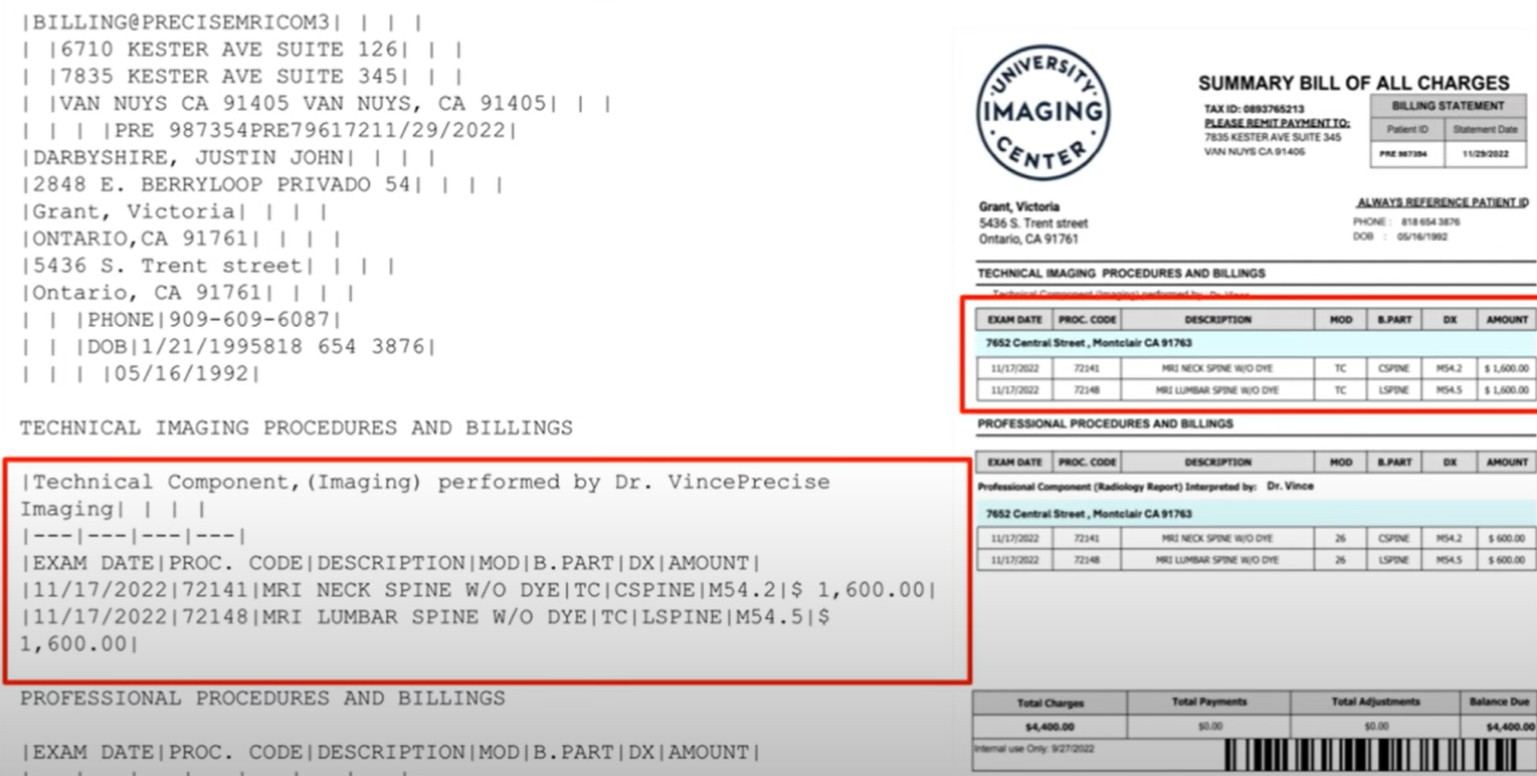
\includegraphics[width=0.8\linewidth,keepaspectratio]{rag_parsing7}
    \end{center}

\end{frame}

%%%%%%%%%%%%%%%%%%%%%%%%%%%%%%%%%%%%%%%%%%%%%%%%%%%%%%%%%%%
\begin{frame}[fragile]\frametitle{X-ray Parser: Multimodal Approach}
  \begin{itemize}
    \item Combines vision models with grounding strategies.
    \item Detects tables and layout visually before parsing.
    \item Converts visual structure into usable text format.
    \item Produces reliable and model-friendly outputs.
    \item Especially effective on visually complex documents.
  \end{itemize}
  
    \begin{center}
      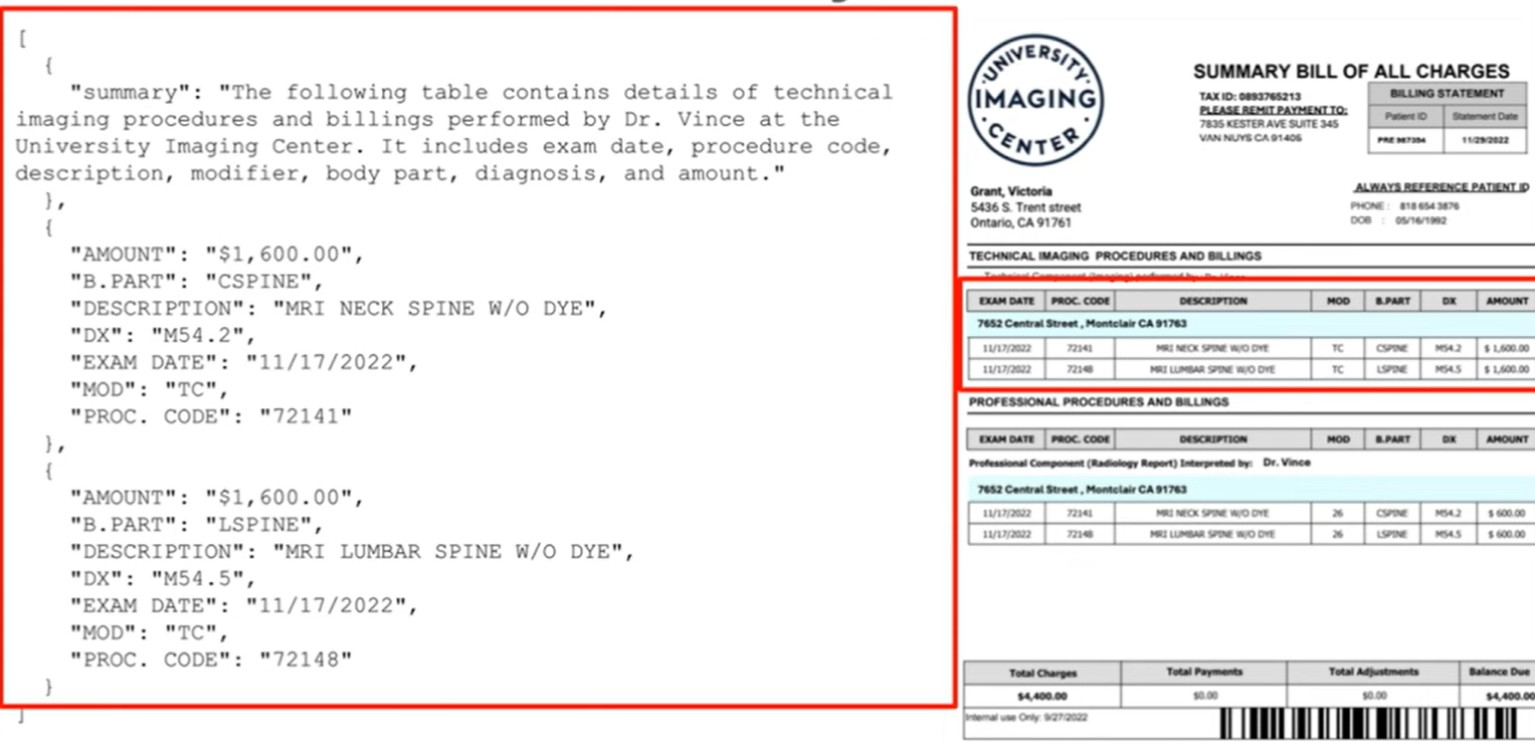
\includegraphics[width=0.8\linewidth,keepaspectratio]{rag_parsing8}
    \end{center}  
\end{frame}

%%%%%%%%%%%%%%%%%%%%%%%%%%%%%%%%%%%%%%%%%%%%%%%%%%%%%%%%%%%
\begin{frame}[fragile]\frametitle{Table Extraction Comparison}

    \begin{itemize}
      \item PyPDF fails with complex tables.
      \item Tesseract detects tables but mangles headers.
      \item Unstructured does OK, but not perfectly.
      \item LlamaParse gives clean markdown tables.
      \item X-ray produces structured, grounded output.
    \end{itemize}

    \begin{center}
      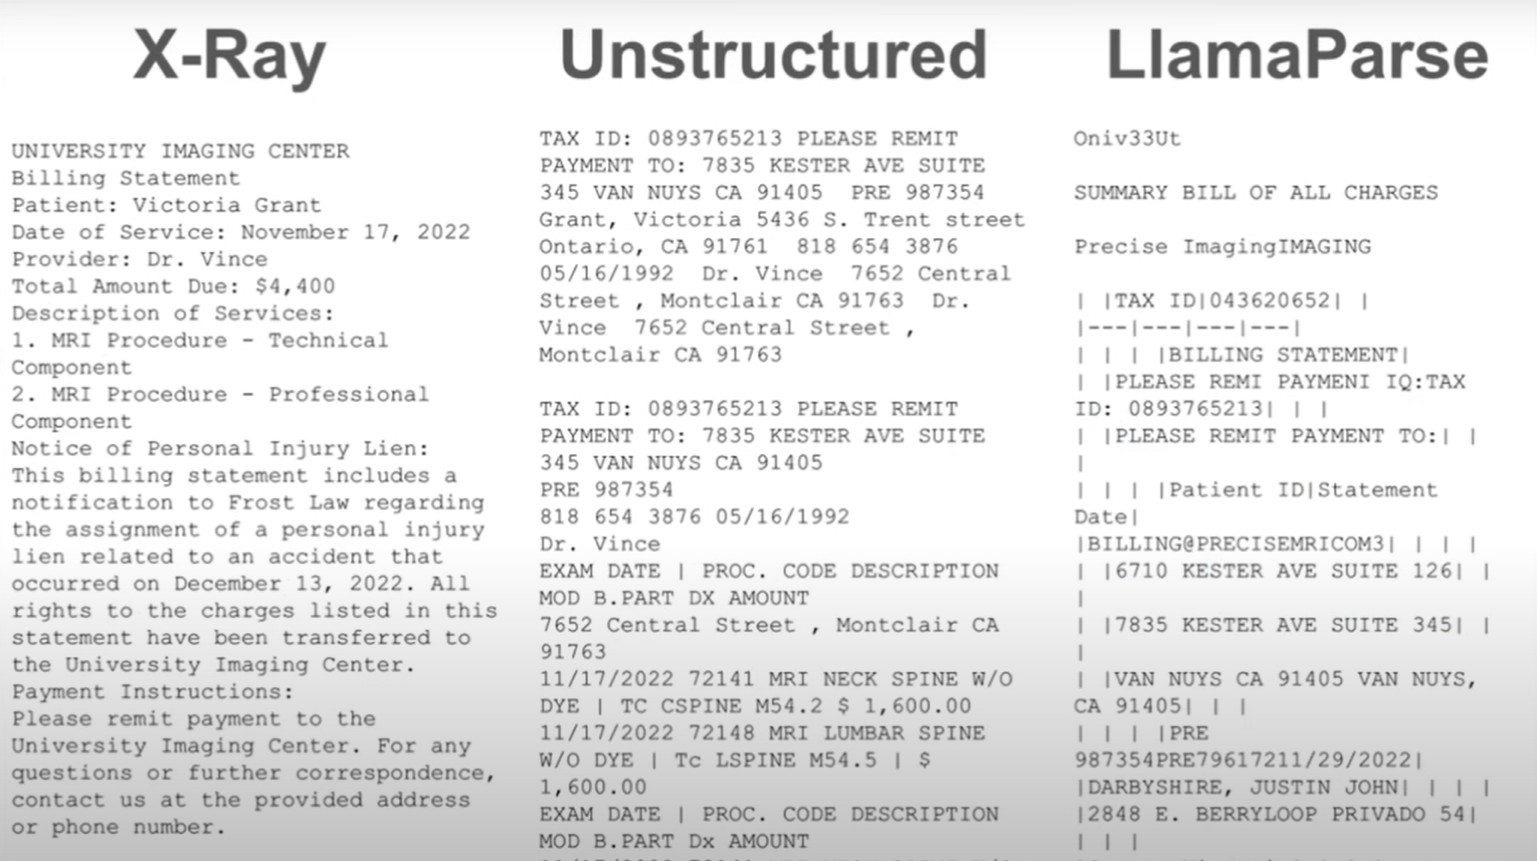
\includegraphics[width=0.8\linewidth,keepaspectratio]{rag_parsing9}
    \end{center}

\end{frame}

%%%%%%%%%%%%%%%%%%%%%%%%%%%%%%%%%%%%%%%%%%%%%%%%%%%%%%%%%%%
\begin{frame}[fragile]\frametitle{Narrative + JSON: A Guided Format}
  \begin{itemize}
    \item Output begins with a narrative summary for context.
    \item Clearly explains the purpose and structure of the table.
    \item Follows with a clean JSON representation of table data.
    \item Format: cell-by-cell structured, easy to interpret.
    \item "Tell-then-show" approach improves model comprehension.
  \end{itemize}
\end{frame}

%%%%%%%%%%%%%%%%%%%%%%%%%%%%%%%%%%%%%%%%%%%%%%%%%%%%%%%%%%%
\begin{frame}[fragile]\frametitle{Why Output Format Matters}
  \begin{itemize}
    \item Parsers may extract the same data, but format it differently.
    \item Output style can strongly affect model performance.
    \item JSON and markdown help structure information clearly.
    \item Human-readable structure supports better inference.
    \item Cleaner format = better grounding for language models.
  \end{itemize}
  

\end{frame}

%%%%%%%%%%%%%%%%%%%%%%%%%%%%%%%%%%%%%%%%%%%%%%%%%%%%%%%%%%%
\begin{frame}[fragile]\frametitle{Impact of Parsing Quality}
  \begin{itemize}
    \item We ran the same RAG pipeline over identical documents.
    \item Different parsers resulted in drastically different performance.
    \item Main variable: parsing quality—not model or retriever.
    \item Shows how foundational parsing is to good RAG results.
    \item A poor parser can undermine even advanced models.
  \end{itemize}
  
    \begin{center}
      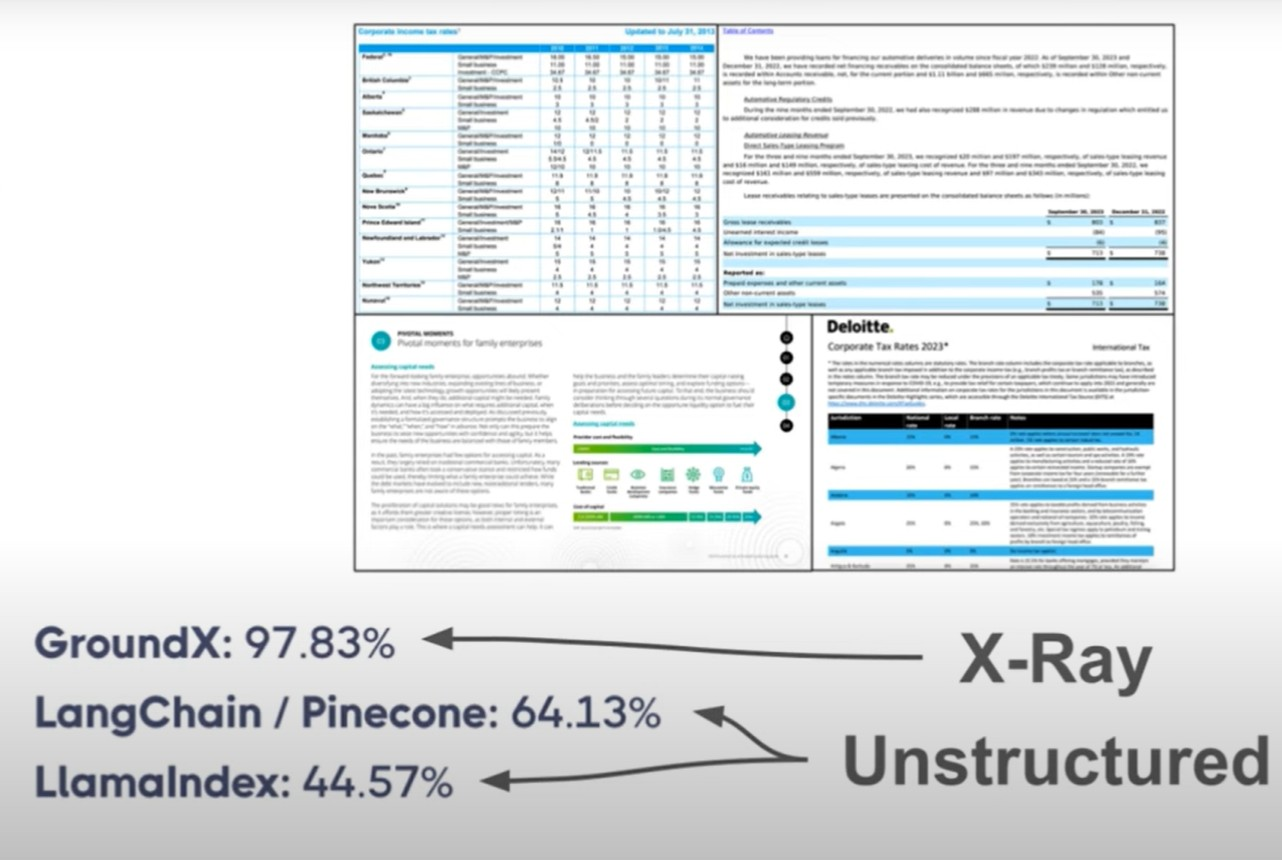
\includegraphics[width=0.6\linewidth,keepaspectratio]{rag_parsing10}
    \end{center}   
\end{frame}

%%%%%%%%%%%%%%%%%%%%%%%%%%%%%%%%%%%%%%%%%%%%%%%%%%%%%%%%%%%
\begin{frame}[fragile]\frametitle{Benchmark Setup (Clarified)}
  \begin{itemize}
    \item \textbf{LlamaIndex}: Used PyPDF (not LlamaParse).
    \item \textbf{LangChain + Pinecone}: Used Unstructured.
    \item \textbf{GroundX}: Used X-ray with vision + grounding.
    \item All pipelines ran the same questions on same documents.
    \item Parser choice significantly influenced accuracy.
  \end{itemize}
  
    \begin{center}
      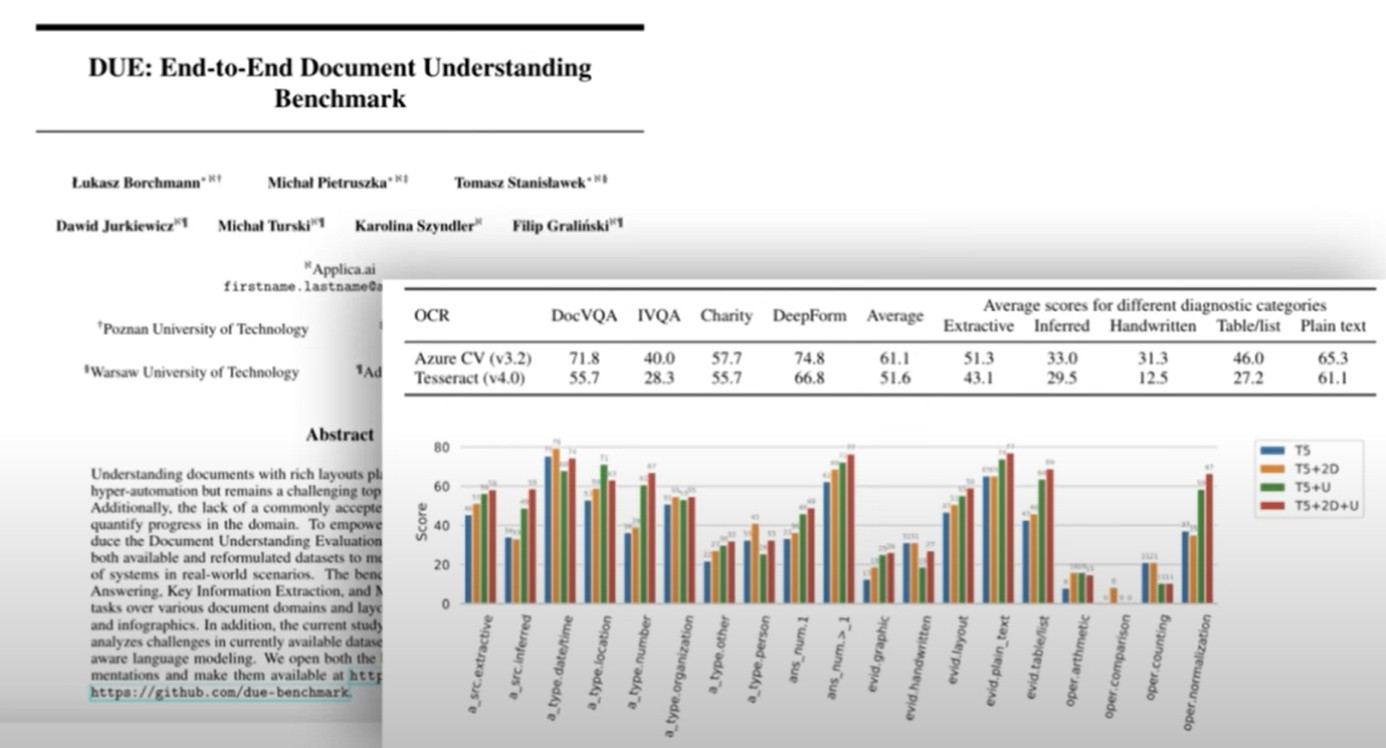
\includegraphics[width=0.8\linewidth,keepaspectratio]{rag_parsing11}
    \end{center}    
\end{frame}


%%%%%%%%%%%%%%%%%%%%%%%%%%%%%%%%%%%%%%%%%%%%%%%%%%%%%%%%%%%
\begin{frame}[fragile]\frametitle{}
\begin{columns}
    \begin{column}[T]{0.5\linewidth}
		Future Test Considerations
		  \begin{itemize}
			\item Results likely to improve if LlamaParse replaces PyPDF.
			\item Parsing upgrades often outperform model upgrades.
			\item Models can only reason with what they’re given.
			\item Better structured data = better answers, less guessing.
			\item Parsing is the cheapest way to level up your RAG stack.
		  \end{itemize}

    \end{column}
    \begin{column}[T]{0.5\linewidth}  
  
		Parsing Alone Can Move the Needle
		  \begin{itemize}
			\item Academia confirms: changing only the parser impacts performance.
			\item Benchmark: same RAG system, different parsers → up to 20-point difference.
			\item Parser quality matters more than fancy downstream techniques.
			\item Quick wins: swap out low-quality parsers before tweaking your RAG logic.
		  \end{itemize}
    \end{column}
  \end{columns}  
   
\end{frame}

%%%%%%%%%%%%%%%%%%%%%%%%%%%%%%%%%%%%%%%%%%%%%%%%%%%%%%%%%%%
\begin{frame}[fragile]\frametitle{Document Context is Crucial}
  \begin{itemize}
    \item Not all documents are created equal.
    \item Scientific papers, 10-Ks, clinical notes – all behave differently.
    \item Choose a parser suited to your specific domain.
    \item No single parser wins for all use cases.
  \end{itemize}
\end{frame}

%%%%%%%%%%%%%%%%%%%%%%%%%%%%%%%%%%%%%%%%%%%%%%%%%%%%%%%%%%%
\begin{frame}[fragile]\frametitle{PDF Parsing Guide}

    \begin{center}
      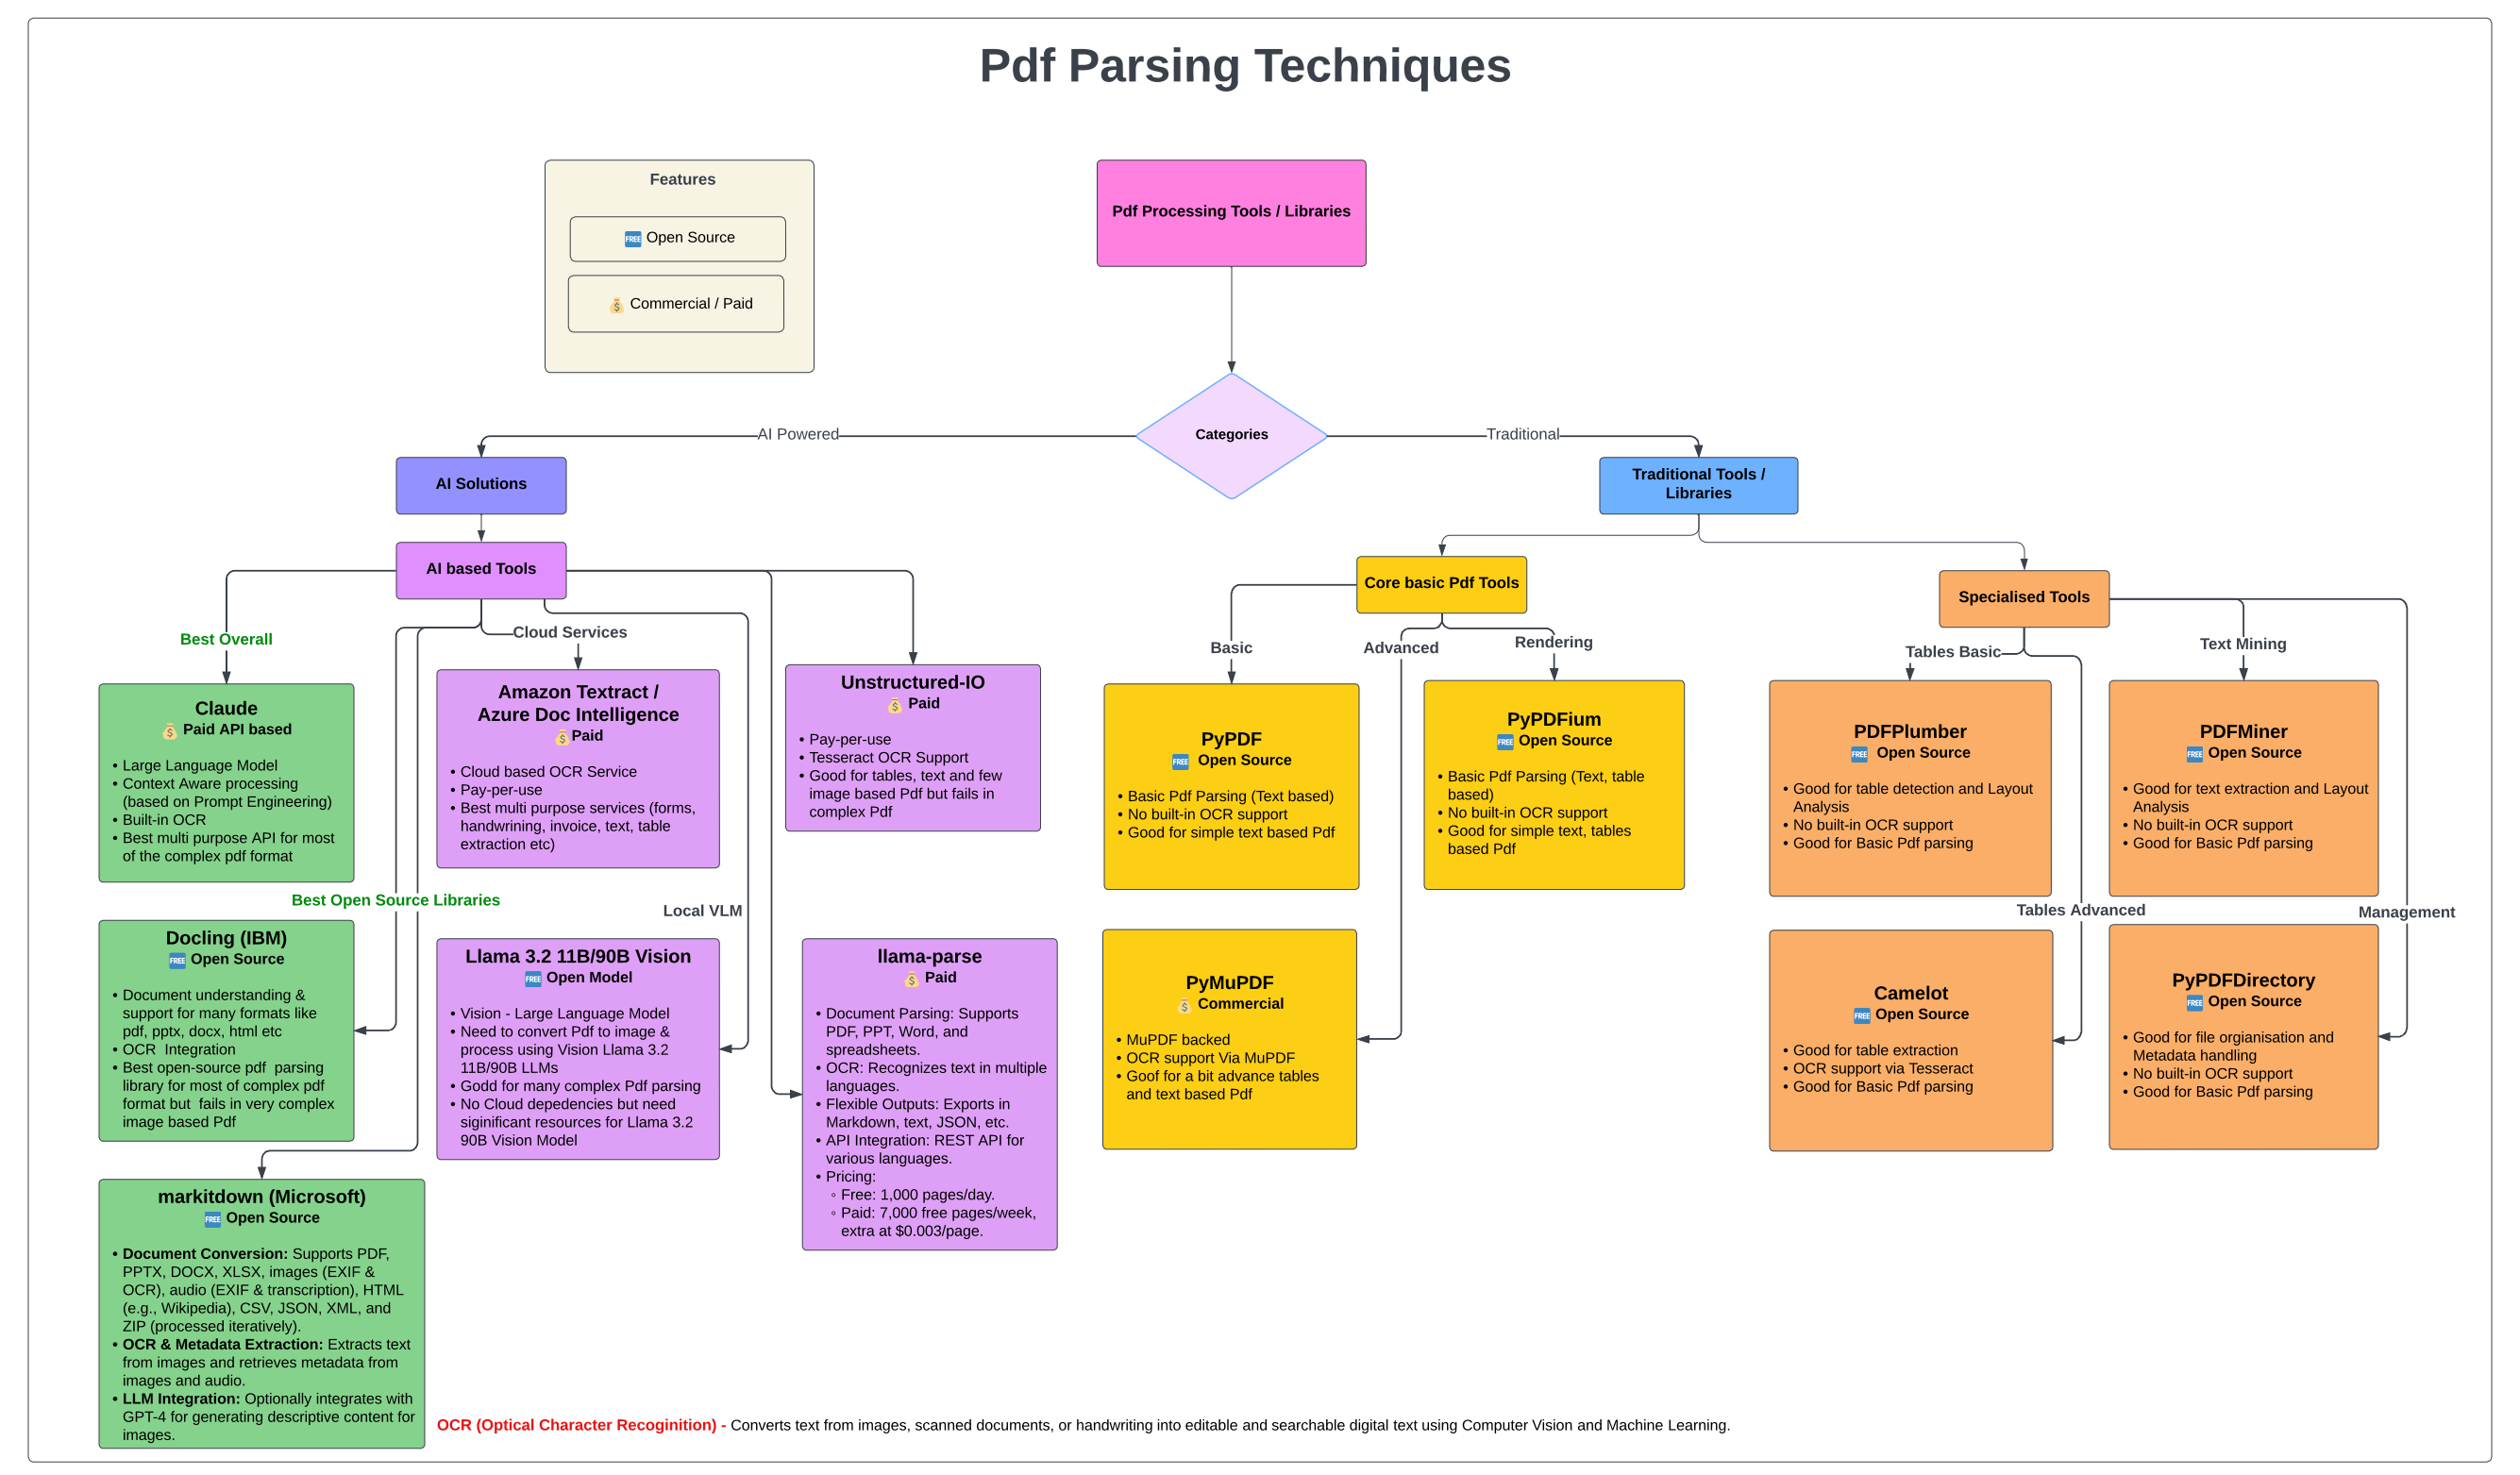
\includegraphics[width=0.8\linewidth,keepaspectratio]{rag_parsing15}
	  
	  {\tiny (Ref: https://github.com/genieincodebottle/parsemypdf/blob/main/pdf-parsing-guide.pdf)}
    \end{center}    
\end{frame}

%%%%%%%%%%%%%%%%%%%%%%%%%%%%%%%%%%%%%%%%%%%%%%%%%%%%%%%%%%%
\begin{frame}[fragile]\frametitle{Picking a Parser: A Two-Pronged Approach}
  \begin{enumerate}
    \item \textbf{Vibe check}: Run your data through multiple parsers. Look at the outputs.
    \item \textbf{End-to-end eval}: Keep the RAG system constant, vary only the parser, then compare results.
  \end{enumerate}
  \vspace{1em}
  \textit{``Your brain is the best model—start with your eyes.''}
  
    \begin{center}
      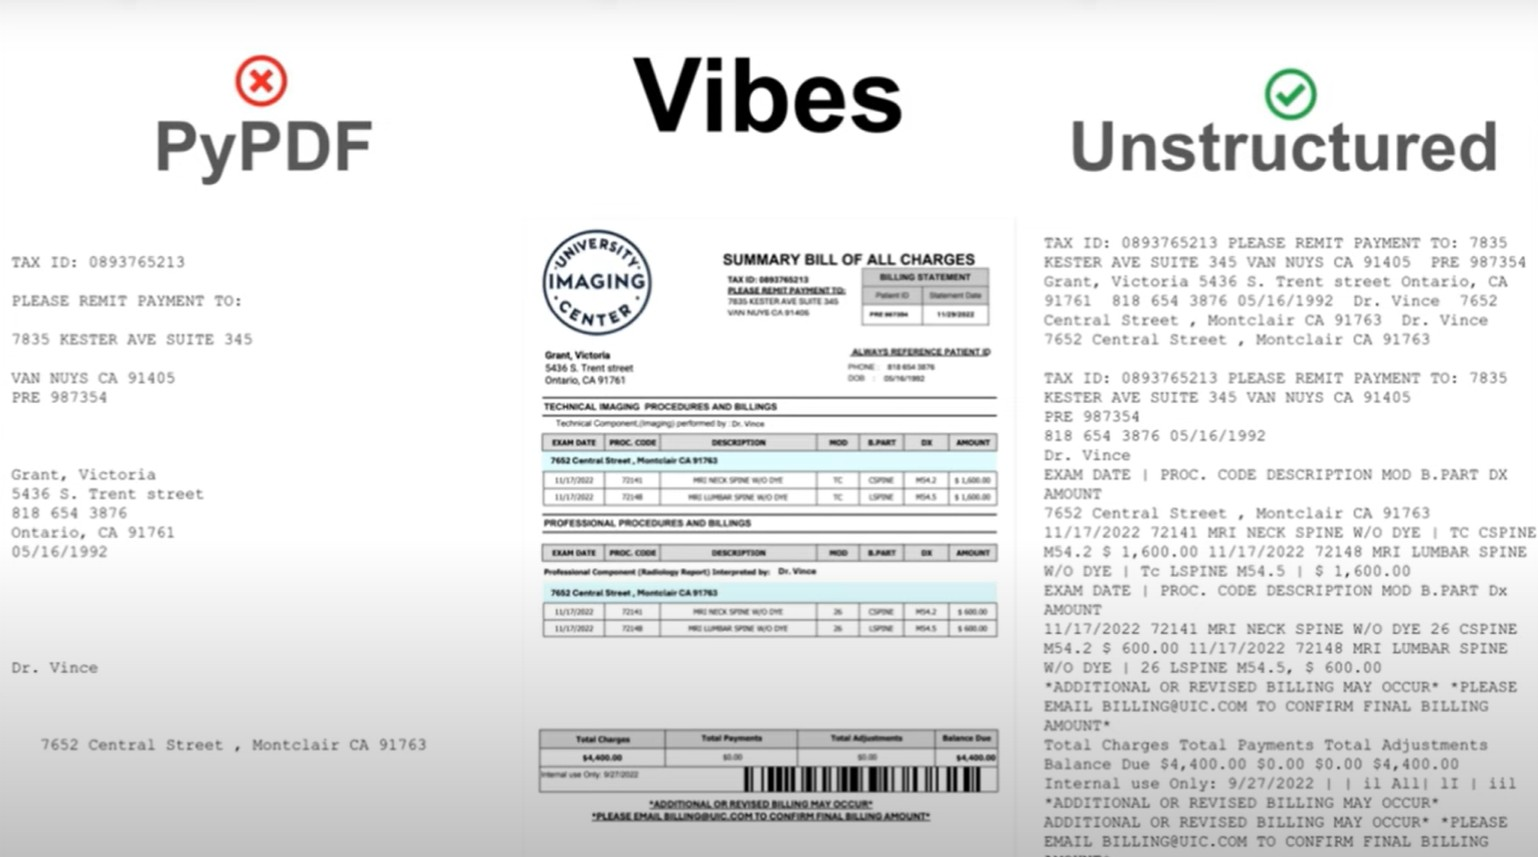
\includegraphics[width=0.8\linewidth,keepaspectratio]{rag_parsing12}
    \end{center}    
\end{frame}

%%%%%%%%%%%%%%%%%%%%%%%%%%%%%%%%%%%%%%%%%%%%%%%%%%%%%%%%%%%
\begin{frame}[fragile]\frametitle{How to Run an End-to-End Evaluation}
  \begin{itemize}
    \item Change one component: the parser.
    \item Keep the rest of the RAG pipeline fixed.
    \item Feed questions through each parser’s output.
    \item Compare generated answers to ground truth.
    \item Labor-intensive, but the most reliable evaluation method.
  \end{itemize}
  
    \begin{center}
      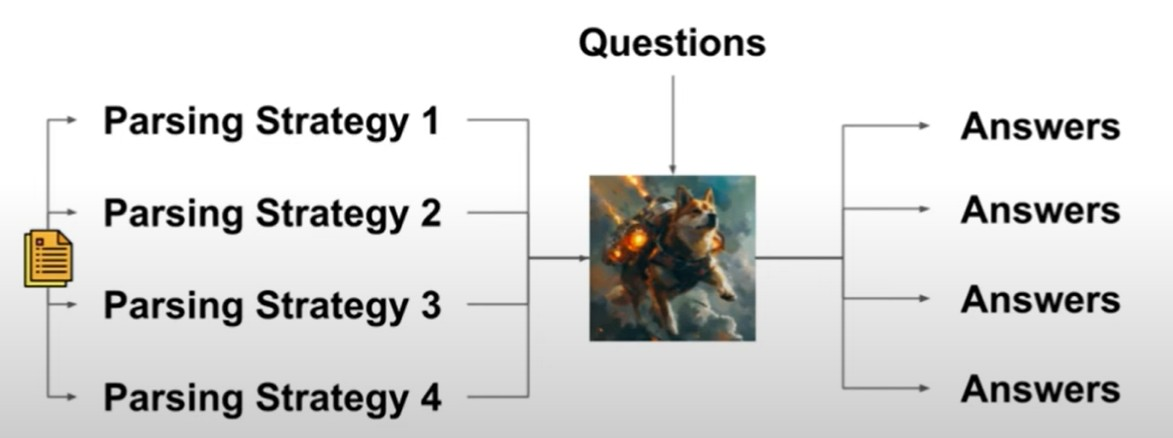
\includegraphics[width=0.7\linewidth,keepaspectratio]{rag_parsing13}
	  
      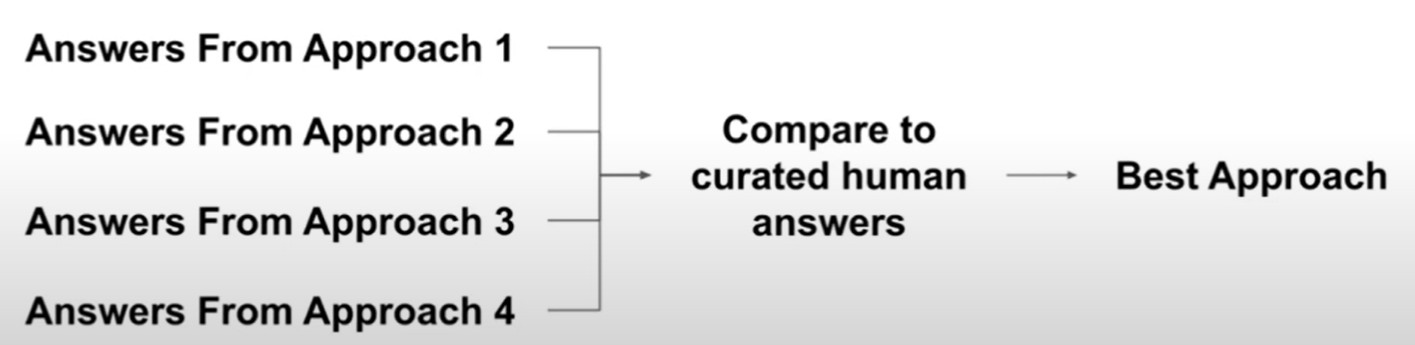
\includegraphics[width=0.8\linewidth,keepaspectratio]{rag_parsing14}
	  
    \end{center}   
\end{frame}

%%%%%%%%%%%%%%%%%%%%%%%%%%%%%%%%%%%%%%%%%%%%%%%%%%%%%%%%%%%
\begin{frame}[fragile]\frametitle{Evaluation}

\begin{columns}
    \begin{column}[T]{0.5\linewidth}
	Auto-Eval: A Helping Hand
	  \begin{itemize}
		\item Start with human-generated QA pairs (ground truth).
		\item Use LLMs to compare parser outputs to ground truth answers.
		\item Helps scale eval, but still requires initial human input.
		\item Avoids the trap of ``models grading their own homework.''
	  \end{itemize}
     
    \end{column}
    \begin{column}[T]{0.5\linewidth}  
	
	Alternative Eval: ELO Ranking
	  \begin{itemize}
		\item Useful when answers are subjective or non-falsifiable.
		\item Compare outputs pairwise: ``Which one is better?''
		\item Rank parsers using ELO-style systems (used in chess).
		\item Great for stylistic or qualitative tasks.
	  \end{itemize}
    \end{column}
  \end{columns}    
\end{frame}

%%%%%%%%%%%%%%%%%%%%%%%%%%%%%%%%%%%%%%%%%%%%%%%%%%%%%%%%%%%
\begin{frame}[fragile]\frametitle{Final Takeaways}
\begin{columns}
    \begin{column}[T]{0.5\linewidth}
  \begin{itemize}
    \item \textbf{Parsing is foundational.} Bad parsing = bad RAG, no matter the model.
    \item \textbf{There is no one-size-fits-all parser.}
    \item \textbf{Evaluate in context.} Use real documents and real questions.
    \item \textbf{Combine human intuition with structured evals.}
    \item \textbf{Opportunities exist.} Big gap in parser testing and tooling.
  \end{itemize}
    \end{column}
    \begin{column}[T]{0.5\linewidth}  
	
  \begin{itemize}
    \item Parsing is hard, but absolutely critical.
    \item Tools like LlamaParse, Unstructured, and X-ray are changing the game.
    \item Try multiple parsers and test thoroughly on your data.
    \item Don’t trust models to validate their own output.
    \item Huge room for innovation in parser evaluation and automation.
  \end{itemize}
    \end{column}
  \end{columns}   
  
\end{frame}

